\section{Three dynamics on one arithmetic}\label{sec:three}

Three different dynamical systems live on the same arithmetic of the moves $U_N,D_N$.

\begin{enumerate}[label=(\Roman*),itemsep=2pt]
\item \emph{Forward arithmetic.} Only up-moves $x\mapsto xr_N$ are used. Every forward path is strictly increasing, so there is no periodic directed orbit, and in every finite subgraph forward paths have bounded length (Proposition~\ref{prop:forward}); on $F_m$ the length is at most $2$.
\item \emph{Autonomous prime-valuation selection.} A deterministic selector chooses one move at each step from the current valuation data. For the selector $\MAXPP$ of the companion paper~\cite{PD} the resulting symbolic sequence is Sturmian: its factor complexity is $p(k)=k+1$, so its entropy is $0$.
\item \emph{Reversible graph histories.} All admissible moves, in both directions, with immediate reversal forbidden: the NB shift $X_{\mathrm{NB}}(G)$. This is a non-deterministic system, and its finite subsystems $X_{\mathrm{NB}}(F_m)$ have entropy $\log\lambda_m\ge\tfrac13\log m$ (Theorem~\ref{thm:capacity}).
\end{enumerate}

\begin{figure}[H]
\centering
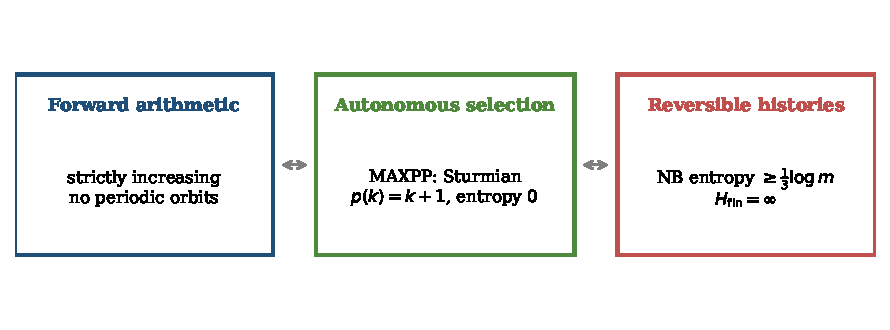
\includegraphics[width=0.96\textwidth]{../figures/fig9_three_dynamics.pdf}
\caption{Three dynamics on the same arithmetic graph: forward arithmetic (no periodic orbits), autonomous selection (Sturmian, zero entropy), reversible NB histories (positive and unboundedly large entropy).}\label{fig:three}
\end{figure}

\begin{proposition}[Deterministic mechanisms have zero entropy]\label{prop:mech}
Let $S$ be a finite set, $f:S\to S$ a map and $o:S\to\mathcal A$ an output map; run the mechanism from every initial state $s_0\in S$ and record the output word $o(s_0)o(f(s_0))o(f^2(s_0))\cdots$. For every $n$ there are at most $|S|$ distinct output words of length $n$; hence the language has zero entropy.
\end{proposition}
\noindent\emph{Source.} The same statement is Proposition E5 of U4-M2-ENT~\cite{UENT}; the proof given here is self-contained.
\begin{proof}
The word of length $n$ is a function of $s_0$. \qedhere
\end{proof}

Proposition~\ref{prop:forward} and Proposition~\ref{prop:mech} locate the source of the entropy. In a finite subgraph, forward histories are finite and any finite-state deterministic selection yields at most $|S|$ words, so no entropy can be produced; the entropy $\log\lambda_m$ of $F_m$ comes entirely from the \emph{freedom of choice among reversible continuations}. In $F_m$ the reversal is what allows a walk to leave a hub along any of $m$ paths and, after traversing it, to turn back at the other hub into any of $m$ paths again (Proposition~\ref{prop:chain}). There is therefore no contradiction between: (I) forward arithmetic has no periodic orbits; (II) the autonomous selector has zero entropy; and (III) the reversible histories of $G$ have positive, unboundedly large entropy. They are entropies of different path spaces: a single deterministic trajectory, versus the set of all admissible histories.

\begin{table}[H]
\centering\small
\resizebox{\textwidth}{!}{\begin{tabular}{lccc}
\toprule
 & forward arithmetic & autonomous selection & reversible histories\\\midrule
choice rule & none (all up-moves) & deterministic selector & none (all NB continuations)\\
periodic orbits & none & none ($\MAXPP$ Sturmian) & $\tr B^n$ per period (Thm~\ref{thm:periodic})\\
entropy in a finite window & $0$ & $0$ & $\log\lambda_m$ for $F_m$\\
unbounded over windows & -- & -- & yes ($\Hfin=\infty$)\\\bottomrule
\end{tabular}}
\caption{The three dynamics compared.}
\end{table}

\section{Reconciliation with the inherited construction}\label{sec:recon}

The inherited release~\cite{UENT} defines $F(x)$ exactly as in Section~\ref{sec:F}, defines the metric shift $Y_{\mathrm{NB}}$ on the induced window, proves $\hNB(F(x))\ge\tfrac14\log(\tau(x)-1)$ (Theorem E1 there; so $\hNB(F(2^m))\ge\tfrac14\log m$), and records numerical spectral radii of its pair-state matrices ($2(3m+1)$ states) for $m=2,\dots,9$ together with Collatz--Wielandt certified lower bounds. We compare these entries with the new formula, without re-running the inherited verifier.

\begin{table}[H]
\centering\small
\begin{tabular}{rrrrr}\toprule $m$ & $\rho$ (inherited, float) & $\lambda_m$ (exact root) & $\tfrac14\log m$-type bound & $\log\lambda_m$\\\midrule
2 & 1.3532099642 & 1.3532099642 & 0.173287 & 0.302480\\
3 & 1.5747430739 & 1.5747430739 & 0.274653 & 0.454092\\
4 & 1.7429592022 & 1.7429592022 & 0.346574 & 0.555584\\
5 & 1.8812394011 & 1.8812394011 & 0.402359 & 0.631931\\
6 & 2.0000000000 & 2.0000000000 & 0.447940 & 0.693147\\
7 & 2.1048727857 & 2.1048727857 & 0.486478 & 0.744255\\
8 & 2.1992803147 & 2.1992803147 & 0.519860 & 0.788130\\
9 & 2.2854733518 & 2.2854733518 & 0.549306 & 0.826573\\
\bottomrule\end{tabular}

\caption{Inherited numerical spectral radius of $Y_{\mathrm{NB}}(F(2^m))$ against the exact root $\lambda_m$ (agreement to $10^{-12}$ in each row), the inherited bound $\tfrac14\log m$ and $\log\lambda_m$.}\label{tab:inherited}
\end{table}

All eight rows agree with $\lambda_m$ to $10^{-12}$; each inherited certified lower bound lies below $\lambda_m$; the inherited state count $2(3m+1)$ equals $|\vec E(F_m)|$; and Theorem~\ref{thm:induced} shows that the agreement is not accidental: the induced window is $F_m$ itself, so the pair-state matrix is the edge matrix $B_{F_m}$. The formula $\hNB(F_m)=\log\lambda_m$ is therefore consistent with the frozen construction and improves its lower bound from $\tfrac14\log m$ to $\tfrac13\log m$ and shows it is sharp up to the additive error $\tfrac1{3m^{1/3}}$. For composite $x$ with $\tau(x)-1=b$ the same value $\log\lambda_b$ is the entropy of the subgraph $F(x)$; the induced window of $F(x)$ is not treated here.

\section{Synthesis}\label{sec:synthesis}

\begin{figure}[H]
\centering
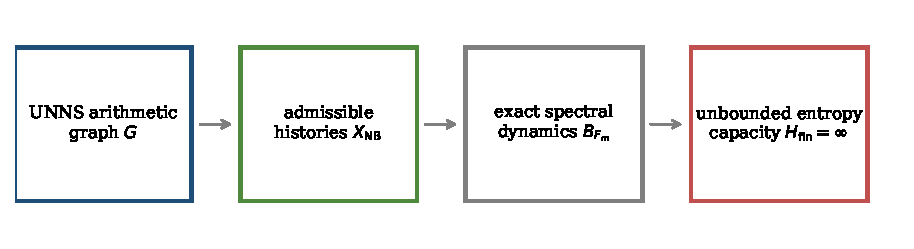
\includegraphics[width=0.98\textwidth]{../figures/fig11_pipeline.pdf}
\caption{The progression established in this paper.}\label{fig:pipeline}
\end{figure}

\paragraph{From the graph to its histories.} The arithmetic graph $G$ is determined by the single family of ratios $r_N=(N+1)^2/N$; its cycles are the realisable multiplicative relations among them (Proposition~\ref{prop:relations}), and its shortest cycles include the scaling squares of Theorem~\ref{thm:cycles}(iv), which provide the explicit family used to construct the subgraphs $F(x)$. Gluing the $\tau(x)-1$ scaling squares at a common edge produces the book graph $F(x)$, a theta graph $\Theta(1,3^{\tau(x)-1})$ sitting inside $G$ as a subgraph, and for $x=2^m$ also as an induced subgraph.

\paragraph{From histories to exact spectral dynamics.} The admissible reversible histories of such a book graph form an edge shift whose entropy is the logarithm of the root of $\sum_i(\lambda^{\ell_i}+1)^{-1}=1$, i.e.\ $\lambda^3-\lambda^2+\lambda=m$. The same computation gives the complete spectrum, the Ihara-type determinant, every periodic-orbit count, the maximal-entropy measure and its stationary distribution, the subdominant spectrum $\sqrt{m/\lambda_m}$, and the comparison with the all-length-$3$ theta graph, whose entropy $\tfrac13\log m$ is the lower bound for $\log\lambda_m$ (Corollary~\ref{cor:theta}).

\paragraph{From exact spectra to unbounded capacity.} Because $\tau(x)$ is unbounded, the finite subsystems $X_{\mathrm{NB}}(F(x))$ have unbounded entropy: $\Hfin(G)=+\infty$, and every sufficiently large window $G[1,X]$ carries entropy at least $\log\lambda_{\tau(x)-1}$ for any $x$ with $4(x+1)^2\le X$. The entropy is produced entirely by reversible freedom of continuation. Forward arithmetic has no periodic orbits and bounded forward length in every finite subgraph, and any deterministic finite-state selection of paths has zero entropy (Section~\ref{sec:three}); so the positive, unbounded entropy of the arithmetic graph is an intrinsic property of its path space, not of any selection rule imposed on it.
